\section{Results}
\label{sec:results}

\subsection{Navigability Estimation Performance}

All four architectures recover navigability well above chance from raw
$32\times24$ tiles, and Feature Fusion leads in every camera direction
(Fig.~\ref{fig:arch_f1}). On validation, Feature Fusion attains overall
per-class $F_1$ of about $0.81$ (\textit{clear}), $0.83$ (\textit{person}),
and $0.80$ (\textit{other object}). The stitched-panorama and output-fusion baselines sit near $0.73$--$0.78$ overall and are weakest on person detection from the right camera.



\subsection{Fusion Strategy Analysis}

Feature-level fusion outperforms both pixel-level stitching and decision-level
output fusion. Concatenating feature maps across cameras at each backbone level
preserves spatial cues that stitching discards in the warp and that output
fusion never observes, since it merges only logits. Feature Fusion requires
additional backbone passes, but at this tile size the accuracy gain justifies
its use in the shuffle experiments below. On a single-sample CPU forward pass,
Model~1, Model~2, and Feature Fusion take 1.36, 0.80, and 2.37\,ms,
respectively, and the camera-identity classifier adds a further 0.21\,ms.
Every configuration remains under 3\,ms, comfortably within budget for
real-time inference on a wearable device.

\subsection{Camera Arrangement Robustness}
\begin{figure}[!t]
    \centering
  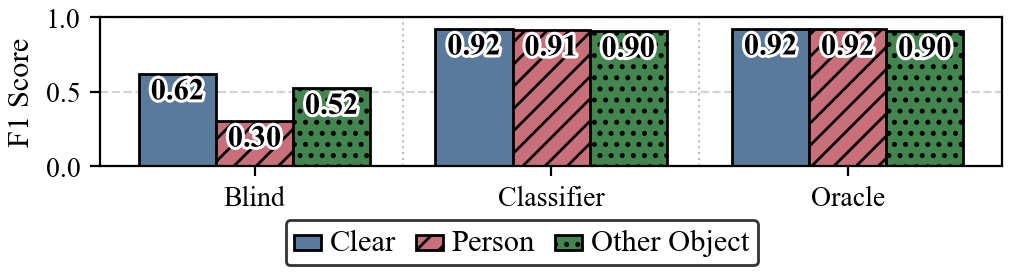
\includegraphics[width=0.9\linewidth]{figs/fig4.png}
  \caption{Overall per-class $F_1$ of Feature Fusion with shuffle correction
  (FF + Shuffle) on the held-out test set (988 frames, not seen during
  training or validation), under blind, classifier, and oracle re-sorting.}
  \label{fig:ff_shuffle}
\end{figure}


Shuffling camera slots collapses uncorrected Feature Fusion, and the
lightweight identity classifier restores it to near-oracle accuracy on the
held-out test set (Fig.~\ref{fig:ff_shuffle}). With no correction (blind),
overall per-class $F_1$ drops to $0.62$ (\textit{clear}), $0.30$
(\textit{person}), and $0.52$ (\textit{other object}), because the fixed-order
projection layers in Model~3 encode slot position. The camera-identity
classifier used to undo this reaches 98.7\% accuracy on the 3-way
slot-identification task on the same 988-frame held-out test set, against a
33.3\% random-guess baseline. Re-sorting the tiles with this classifier before
inference recovers an overall $F_1$ of approximately $0.90$--$0.92$ across all
three classes, matching the ground-truth-identity oracle to within rounding.
The backbone features carry direction information. What breaks under shuffle
is the slot ordering, not the thermal representation itself.